\begin{wrapfigure}[13]{r}{.25\textwidth}
\centering
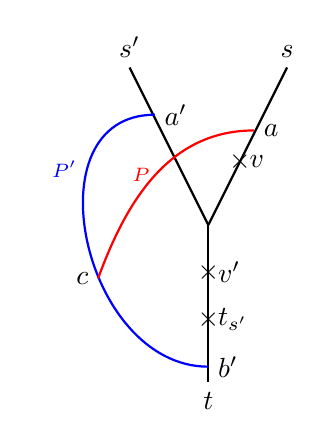
\begin{tikzpicture}[scale=2]
\begin{scope}[xshift=5.1cm]
\coordinate (s) at (-0.5,2);
\coordinate (s1) at (0.5,2);
\coordinate (w) at (0,1);
\coordinate (t) at (0,0);
\coordinate (ts) at (0,0.4);
\coordinate (b1) at (0,0.1);

\coordinate (i1) at (-0.265,1.5);
\coordinate (i2) at (-0.1,1.2);

\coordinate (a1) at (-0.34,1.7);
\coordinate (a) at (0.29,1.6);
\coordinate (v) at (0.2,1.4); 
\coordinate (v1) at (0,0.7); 
\coordinate (c) at (-0.7,0.66); 

\draw[thick](s)--(w);
\draw[thick](s1)--(w);
\draw[thick](w)--(t);
\node[above] at (s){$s'$};
\node[above] at (s1){$s$};
\node[below] at (t){$t$};
\node[right] at (a1){$a'$};
\node[right] at (a){$a$};
\node[right] at (b1){$b'$};
\node[left] at (c){$c$};


\draw[blue,thick] (a1) to[out=180,in=180,distance=.8cm]
node[pos=0.3,left]
{\scriptsize  $P'$}  (b1);

\draw[red,thick] (a) to[out=180,in=70]
node[pos=0.6,above]
{\scriptsize  $P$}  (c);

\node at (v1){$\times$};
\node[right] at (v1){$v'$};

\node at (v){$\times$};
\node[right] at (v){$v$};

\node at (ts){$\times$};
\node[right] at (ts){$t_{s'}$};

\end{scope}
\end{tikzpicture}
\caption{ffs}
\label{fig:badexample2}

\end{wrapfigure}
